\input{../preamble.tex}
% \bibliographystyle{plain} % Style BST file (bmc-mathphys, vancouver, spbasic).
% \bibliographystyle{unsrt} % Style BST file (bmc-mathphys, vancouver, spbasic).
\bibliography{pubs.bib}      % Bibliography 

\title{Professional Drone, Hybrid Power Pack  - Timebox 7}
\author{Team 2}

\begin{document}

\lstset{language=C,%
  % basicstyle=\color{red},
  breaklines=true,%
  morekeywords={matlab2tikz},
  keywordstyle=\color{blue},%
  morekeywords=[2]{1}, keywordstyle=[2]{\color{black}},
  identifierstyle=\color{black},%
  stringstyle=\color{mylilas},
  commentstyle=\color{mygreen},%
  showstringspaces=false,%without this there will be a symbol in the places where there is a space
  % numbers=left,%
  % numberstyle={\tiny \color{black}},% size of the numbers
  % numbersep=9pt, % this defines how far the numbers are from the text
  emph=[1]{for,end,break},emphstyle=[1]\color{red}, %some words to emphasise
  % emph=[2]{word1,word2}, emphstyle=[2]{style},    
}
% \lstdefinestyle{customc}{
%   belowcaptionskip=1\baselineskip,
%   breaklines=true,
%   frame=L,
%   xleftmargin=\parindent,
%   language=C,
%   showstringspaces=false,
%   basicstyle=\footnotesize\ttfamily,
%   keywordstyle=\bfseries\color{green!40!black},
%   commentstyle=\itshape\color{purple!40!black},
%   identifierstyle=\color{blue},
%   stringstyle=\color{orange},
% }

% \lstdefinestyle{customasm}{
%   belowcaptionskip=1\baselineskip,
%   frame=L,
%   xleftmargin=\parindent,
%   language=[x86masm]Assembler,
%   basicstyle=\footnotesize\ttfamily,
%   commentstyle=\itshape\color{purple!40!black},
% }

% \lstset{escapechar=@,style=customc}

\newcounter{udrboks}[section]\setcounter{udrboks}{0}
\renewcommand{\theudrboks}{\arabic{section}.\arabic{udrboks}}
\renewcommand{\theudrboks}{\arabic{udrboks}}
\newenvironment{udrboks}[2][]{%
  \refstepcounter{udrboks}%
  \ifstrempty{#1}%
  {\mdfsetup{%
      frametitle={%
        \tikz[baseline=(current bounding box.east),outer sep=0pt]
        \node[anchor=east,rectangle,fill=blue!20]
        {\strut Udregninger~\theudrboks};}}
  }%
  {\mdfsetup{%
      frametitle={%
        \tikz[baseline=(current bounding box.east),outer sep=0pt]
        \node[anchor=east,rectangle,fill=blue!20]
        {\strut Udregninger ~\theudrboks:~#1};}}%
  }%
  \mdfsetup{innertopmargin=10pt,linecolor=blue!20,%
    linewidth=2pt,topline=true,%
    frametitleaboveskip=\dimexpr-\ht\strutbox\relax
  }
  \begin{mdframed}[]\relax%
    \label{#2}}{\end{mdframed}}


\newcounter{formelboks}[section]\setcounter{formelboks}{0}
\renewcommand{\theformelboks}{\arabic{section}.\arabic{formelboks}}
\renewcommand{\theformelboks}{\arabic{formelboks}}
\newenvironment{formelboks}[2][]{%
  \refstepcounter{formelboks}%
  \ifstrempty{#1}%
  {\mdfsetup{%
      frametitle={%
        \tikz[baseline=(current bounding box.east),outer sep=0pt]
        \node[anchor=east,rectangle,fill=blue!20]
        {\strut Formler~\theformelboks};}}
  }%
  {\mdfsetup{%
      frametitle={%
        \tikz[baseline=(current bounding box.east),outer sep=0pt]
        \node[anchor=east,rectangle,fill=blue!20]
        {\strut Formler ~\theformelboks:~#1};}}%
  }%
  \mdfsetup{innertopmargin=10pt,linecolor=blue!20,%
    linewidth=2pt,topline=true,%
    frametitleaboveskip=\dimexpr-\ht\strutbox\relax
  }
  \begin{mdframed}[]\relax%
    \label{#2}}{\end{mdframed}}

\newcounter{konstboks}[section]\setcounter{konstboks}{0}
\renewcommand{\thekonstboks}{\arabic{section}.\arabic{konstboks}}
\newenvironment{konstboks}[2][]{%
  \refstepcounter{konstboks}%
  \ifstrempty{#1}%
  {\mdfsetup{%
      frametitle={%
        \tikz[baseline=(current bounding box.east),outer sep=0pt]
        \node[anchor=east,rectangle,fill=green!20]
        {\strut Konstanter~\thekonstboks};}}
  }%
  {\mdfsetup{%
      frametitle={%
        \tikz[baseline=(current bounding box.east),outer sep=0pt]
        \node[anchor=east,rectangle,fill=green!20]
        {\strut Konstanter~\thekonstboks:~#1};}}%
  }%
  \mdfsetup{innertopmargin=10pt,linecolor=green!20,%
    linewidth=2pt,topline=true,%
    frametitleaboveskip=\dimexpr-\ht\strutbox\relax
  }
  \begin{mdframed}[]\relax%
    \label{#2}}{\end{mdframed}}
\pgfplotstableread[row sep=\\,col sep=&]{
  ide & stemmer  \\
  Paraply & 9  \\
  Fjernbetjening & 7  \\
  iAdapt & 2 \\
}\mydata
% \setcounter{secnumdepth}{1}
\maketitle
\thispagestyle{empty}

\textbf{Deltagere:}
\begin{figure}[h]
  \centering
  % BEGIN RECEIVE ORGTBL delt
  \begin{tabular}{|p{5cm}p{10cm}|}
    \hline
    &\\
    Stud. nr: 201602094 & Navn: Søren Holm Korsgaard \\
    \hline
    &\\
    % Stud.nr.: 201607563 & Navn: Jacob Gustafsson \\
    % \hline
    % &\\
    % Stud.nr.: 201704859 & Navn: Jonas Buus \\
    % \hline
    % &\\
    Stud.nr.: 20084327 & Navn: Simon Rasmussen \\
    \hline
    &\\
    Stud.nr.: 201704483 & Navn: Thomas Dueholm Jensen \\
    \hline
  \end{tabular}
  % END RECEIVE ORGTBL delt

\end{figure}
\vspace{-5mm}
% \clearpage
\setcounter{tocdepth}{2}
\tableofcontents
\thispagestyle{empty}
\newpage
% \pagenumbering{arabic}
\setcounter{page}{1}

% \section{Introduktion}
% \label{sec:introduktion}

\section{Strategy and planning (Thomas)}
\label{sec:strategy-planning}

I perioden mellem Timebox 6 og 7 har der været flere udfordringer, som har forsinket arbejdsplanen en del. Simon Rasmussen er blevet far 4 uger for tidligt ift. termin, hvilket har forårsaget, at arbejdet med PID reguleringen af motoren har været på standby. Thomas Dueholm har ligget syg i ca. 10 dage med børn, hvilket også forsinkede hans arbejde. Jonas Nielsen har meldt ud til gruppen, at han er i samtale med studievejledningen om at få forlænget sit studie, hvilket medfører, at han måske ikke skal deltage i Projekt 4 længere. Dette er dog endnu uopklaret, men Jonas har af denne årsag valgt, at trække sig fra arbejdet med den aktive ensretter.

Disse udfordringer har medvirket til, at der er lavet nogle strukturelle ændringer ift. arbejdsfordelingen og tidsplanen, således der kan leves op til målet med projektet. 

\subsection{Aktiv ensretter}
\label{sec:aktiv-ensretter}

\subsubsection{Strategy}
\label{sec:strategy}

Gruppen har i samråd besluttet, at Søren Korsgaard skal bistå med arbejdet og udviklingen af den aktive ensretter sammen med Thomas Dueholm. Strategien for arbejdet med ensretteren i Timebox 7 vil være at få simuleret det valgte kredsløb til realiseringen vha. programmet, LT-spice. Derudover skal kredsløbet opbygges på breadboard i en nedskaleret version med en load-modstand på 1 k$\Omega$, således der ikke trækkes for stor en strøm. Dette gøres for at vise funktionaliteten af kredsløbet. I denne forbindelse skal der udvikles en ny teststand, hvorved det er muligt at generere en trefaset spænding uden at skulle opstarte forbrændingsmotoren hver gang.

\subsubsection{Deployment plan}
\label{sec:deployment-plan}

I Timebox 7 er det planen, at der skal deployes en ny teststand, som kan generere en trefaset spænding. Dette gør det muligt at teste den aktive ensretter i forskellige niveauer og frekvenser. Der skal ligeledes deployes en simulering af kredsløbet vha. programmet, LT-spice.  Afslutningsvist skal der deployes en nedskaleret version af realiseringen af den aktive ensretter på breadboard. Realiseringen laves for at konstatere, at de tre faser bliver ensrettet, samt at de tre IC’er, LT4320-1, tænder og slukker de tilkoblede MOSFETS korrekt for hver fase.

% \subsection{Spændingsregulator}
% \label{sec:spandingsregulator}

% Jacob Gustavsson har i Timebox 7 arbejdet videre med realiseringen af spændingsregulatoren. Se pågældende afsnit for yderligere information.

% \subsubsection{Deployment plan}
% \label{sec:deployment-plan-1}

\subsection{Motorstyring (PID)}
\label{sec:motorstyring-pid}

Som tidligere nævnt er arbejdet med motorstyringen blevet forsinket på grund af for tidlig fødsel, men gruppen er i samråd med Simon Rasmussen blevet enige, om at det på nuværende tidspunkt ikke er nødvendigt at ændre noget i planlægningen af arbejdet. Simon har givet udtryk for, at han er optimistisk ift. at kunne indhente det tabte arbejde, hvorfor han fortsætter med udviklingen af motorstyring på egen hånd indtil videre.

\subsubsection{Deployment plan}
\label{sec:deployment-plan-2}

I Timebox 7 skal der for motorstyringen deployes et design af teststand til realisering af målinger af koefficienter til PID reguleringen. Når designet er klar, skal der i timebox 8 arbejdes med at fastlægge de mest ideelle koefficienter til motorstyringen. For nærmere information se det pågældende afsnit.

\subsection{Development plan}
\label{sec:development-plan}

Hvis alt går efter planen i denne timebox, skal der i Timebox 8 arbejdes med følgende:
\begin{itemize}
\item PCB print af spændingsregulator.
\item PCB print af aktiv ensretter.
\item Fastlæggelse af koefficienter til PID-regulering.
\end{itemize}

Ved opstart af Timebox 8 vil der blive produceret en mere udførlig planlægning arbejdsindholdet. Figur~\ref{fig:devplan} viser et skærmbillede af development planen for resten af projekt 4.

\begin{figure}[h]
  \centering
  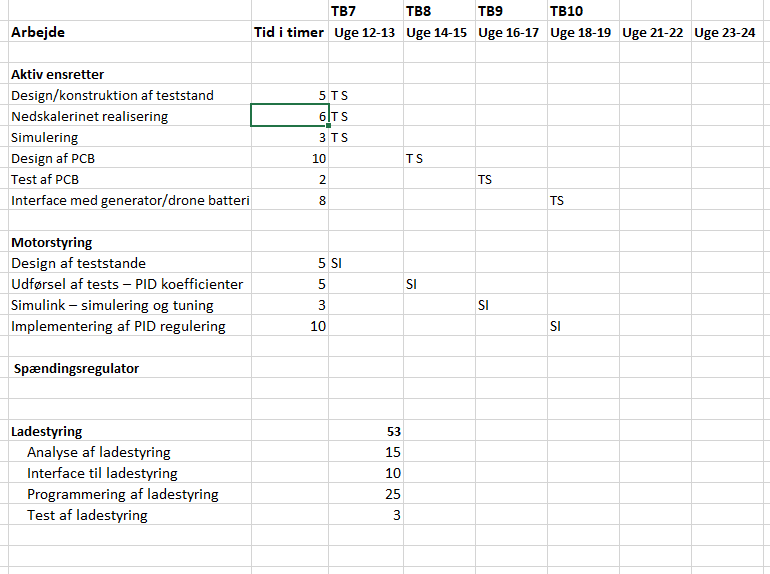
\includegraphics[width=0.5\textwidth]{devplan.png}
  \caption{Development plan}
  \label{fig:devplan}
\end{figure}
\clearpage
\section{Aktive ensretter}
\label{sec:aktive-ensretter}

\subsection{Design og konstruktion af teststand til den aktive ensretter (Thomas)}
\label{sec:design-og-konstr}

I Strategy and Planning for Timebox 7 er det beskrevet, at der skal konstrueres en ny teststand til den aktive ensretter, således det er muligt at generere en trefaset spænding uden opstart af forbrændingsmotoren. Dette afsnit omhandler netop det. Design og konstruktion af lavet af Søren og Thomas.

Da der er behov for at have et setup, hvor der problemløst kan genereres en trefaset spænding til at teste den aktive ensretter, har vi besluttet, at det ikke er sikkerhedsmæssigt forsvarligt indtil videre at benytte forbrændingsmotoren til at drive generatoren. Vi har fra start af været i besiddelse af en ekstra generator, og hvis denne forbindes med den oprindelige generator, vil det derved være muligt at generere en trefaset spænding.

Den oprindelig stand med påmonteret forbrændingsmotor og generator benyttes til den nye teststand. Tandremmen mellem forbrændingsmotor og generatoren afmonteres, hvorefter standen boltes fast til en træ reglar med dimensionerne, 5x10x45 cm. Den ekstra generator boltes fast til en jernplade med to stålklemmer, hvorefter jernpladen påmonteres træ reglaren i passende afstand til den oprindelige generator. Herefter forbindes akslen på de to generatorer med en ny tandrem. I figur~\ref{fig:test1} og~\ref{fig:test2} ses billeder af den færdige teststand. 

\begin{figure}[h]
  \centering
  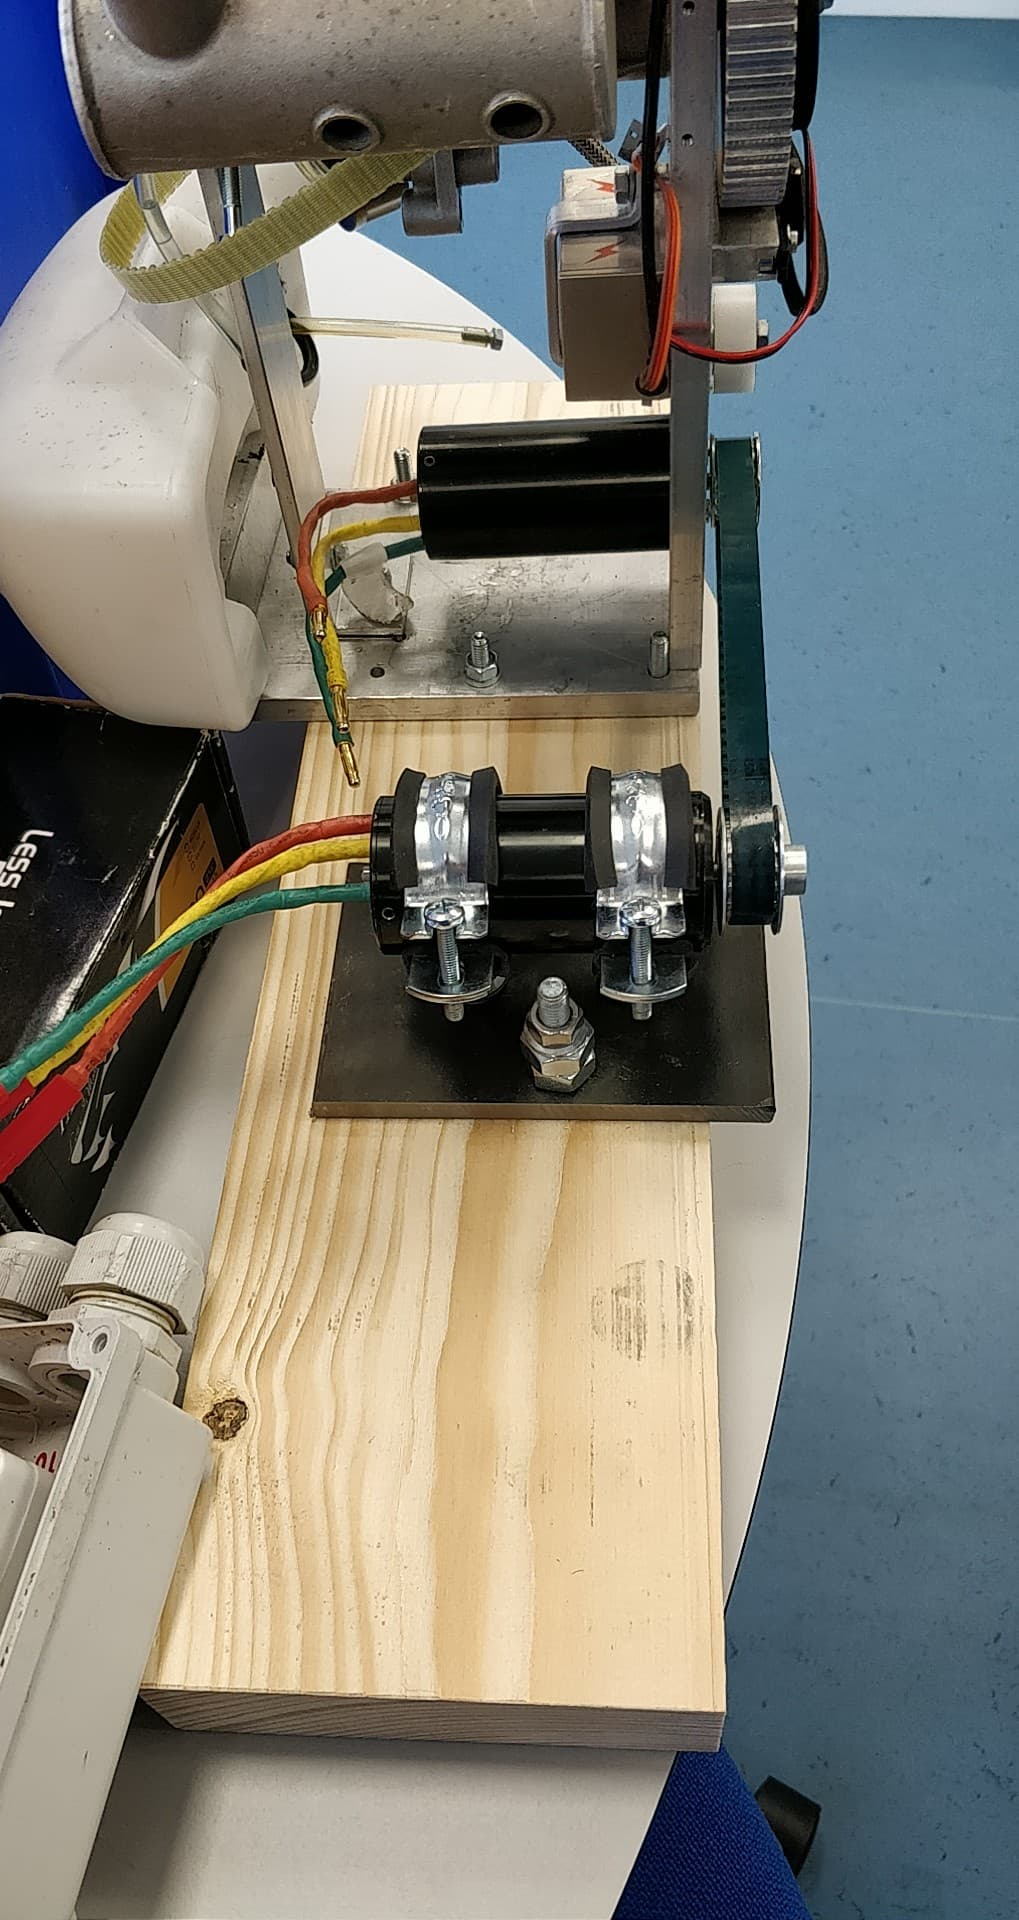
\includegraphics[width=0.4\textwidth]{teststand1.jpg}
  \caption{Foto af teststand til produktion af 3 faset spænding}
  \label{fig:test1}
\end{figure}
\clearpage
\begin{figure}[h]
  \centering
  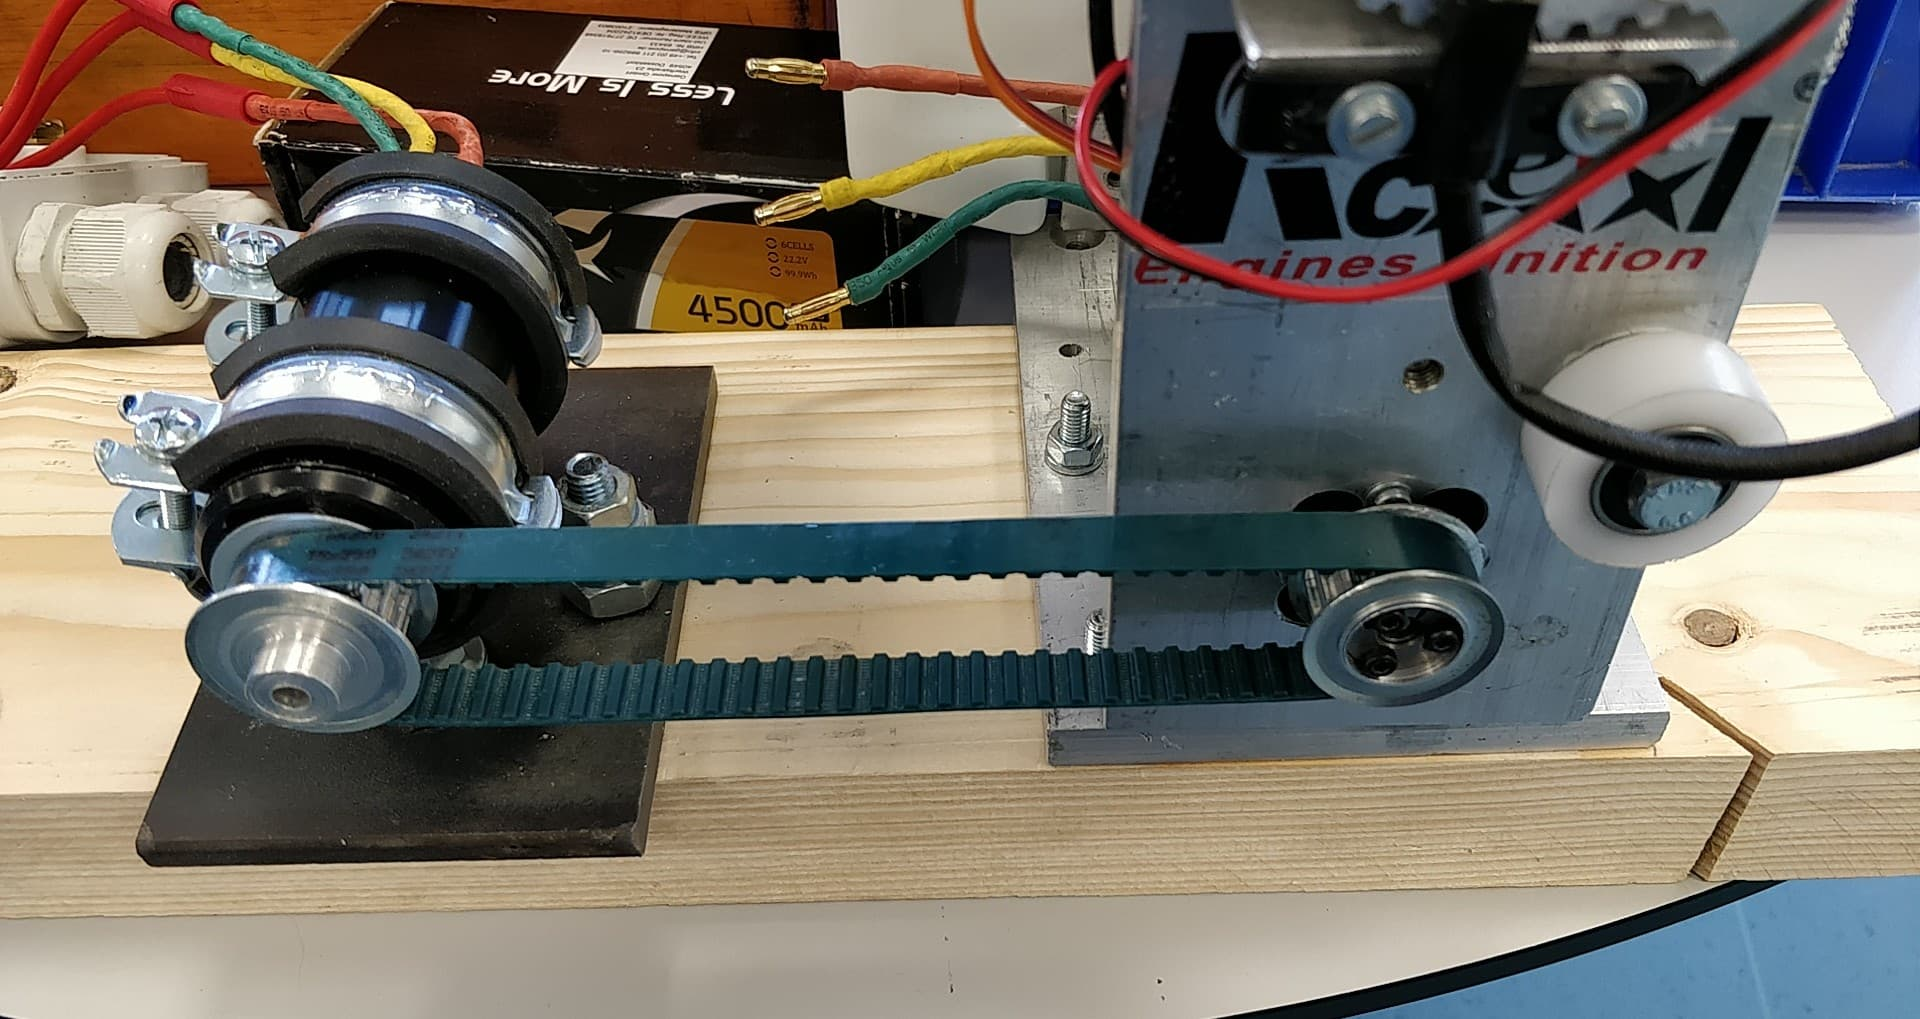
\includegraphics[width=0.8\textwidth]{teststand2.jpg}
  \caption{Foto af teststand til produktion af 3 faset spænding}
  \label{fig:test2}
\end{figure}

Ved hjælp af den tidligere benyttede ESC og kildekode, vil det nu være muligt at starte den nye generator med forskellige frekvenser, hvilket vil give et tilsvarende output på den oprindelige generator. Dette output kan tilkobles den aktive ensretter, således det er muligt at teste dens funktionalitet.
\clearpage
\subsection{Simulering af aktiv ensretter (Thomas)}
\label{sec:simulering-af-aktiv}

Inden vi påbegynder opbygningen af den aktive ensretter med IC’er, LT4320-1, har vi lavet en simulering af kredsløbet vha. simuleringsprogrammet, LT-spice, som er leveret af IC’ens producent\footnote{https://www.analog.com/en/design-center/design-tools-and-calculators/ltspice-simulator.html}. På producentens hjemmeside kan der findes et udarbejdet schematic til det valgte kredsløb, og dette schematic kan benyttes til simuleringen. Figur~\ref{fig:schem} viser et skærmbillede af det simulerede kredsløb.

\begin{figure}[h]
  \centering
  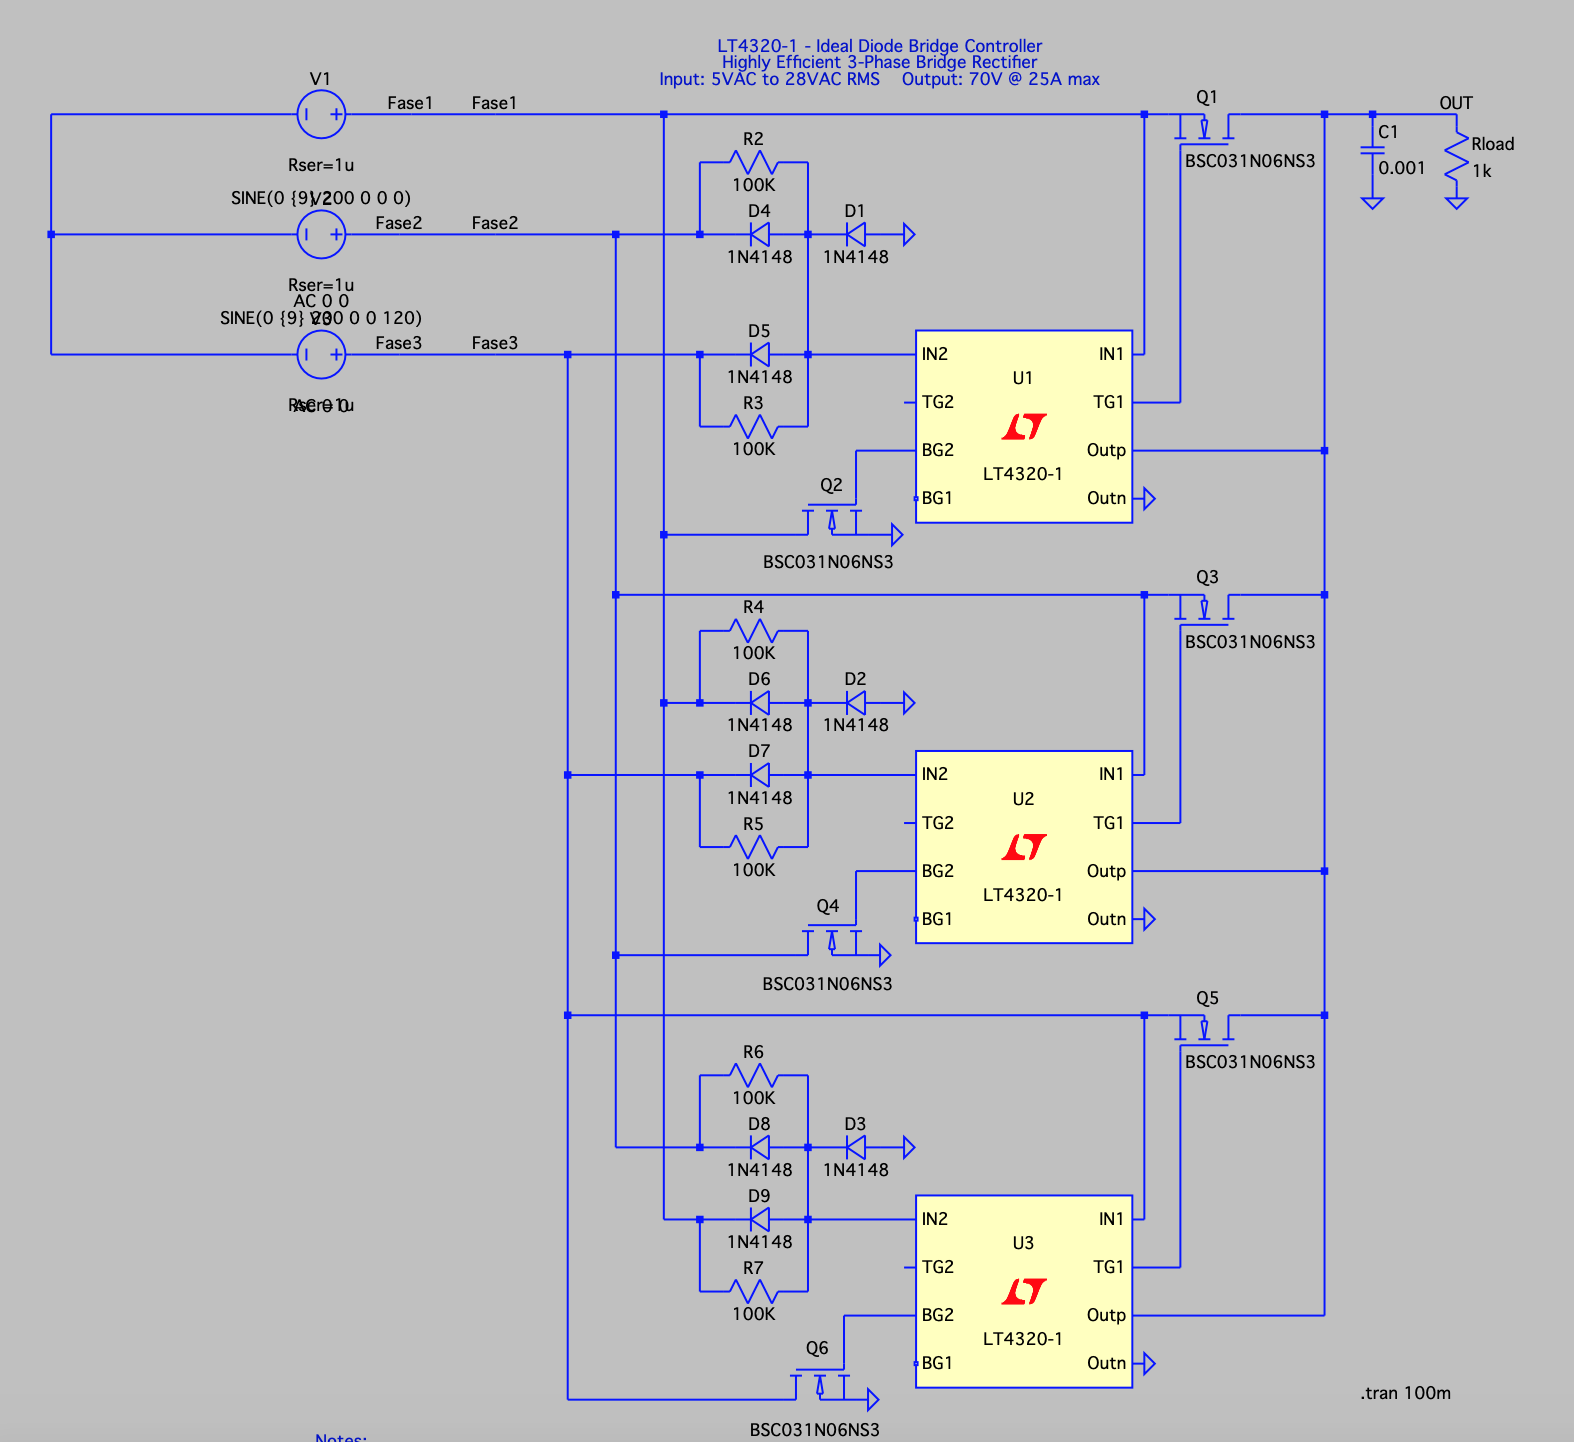
\includegraphics[width=0.6\textwidth]{schem.png}
  \caption{Schematic til aktiv ensretter kredsløb. Måle prober er symboliseret med +/-}
  \label{fig:schem}
\end{figure}

Det er ikke muligt at benytte de samme MOSFETS, som skal bruges til realiseringen af kredsløbet, men det er vurderet, at det ikke har nogen betydning, da simuleringen blot skal bevise den teoretiske funktionalitet af den aktive ensretter. Valg af korrekte MOSFTES har større betydning, når kredsløbet skal skaleres til HPP’s reelle behov. 
Under simuleringen er de tre input faser indstillet til en amplitude på 9 V (peak) og faser på henholdsvis 0, 120 og 240 grader. Load kondensatoren er sat til 1000 $\mu$F og load modstanden er sat til 1 k$\Omega$. Dette er samme værdier, som skal benyttes til realiseringen af det nedskalerede kredsløb på breadboard i det efterfølgende afsnit.
\clearpage
I figur~\ref{fig:real1} ses et skærmbillede af resultatet af realiseringen.

\begin{figure}[h]
  \centering
  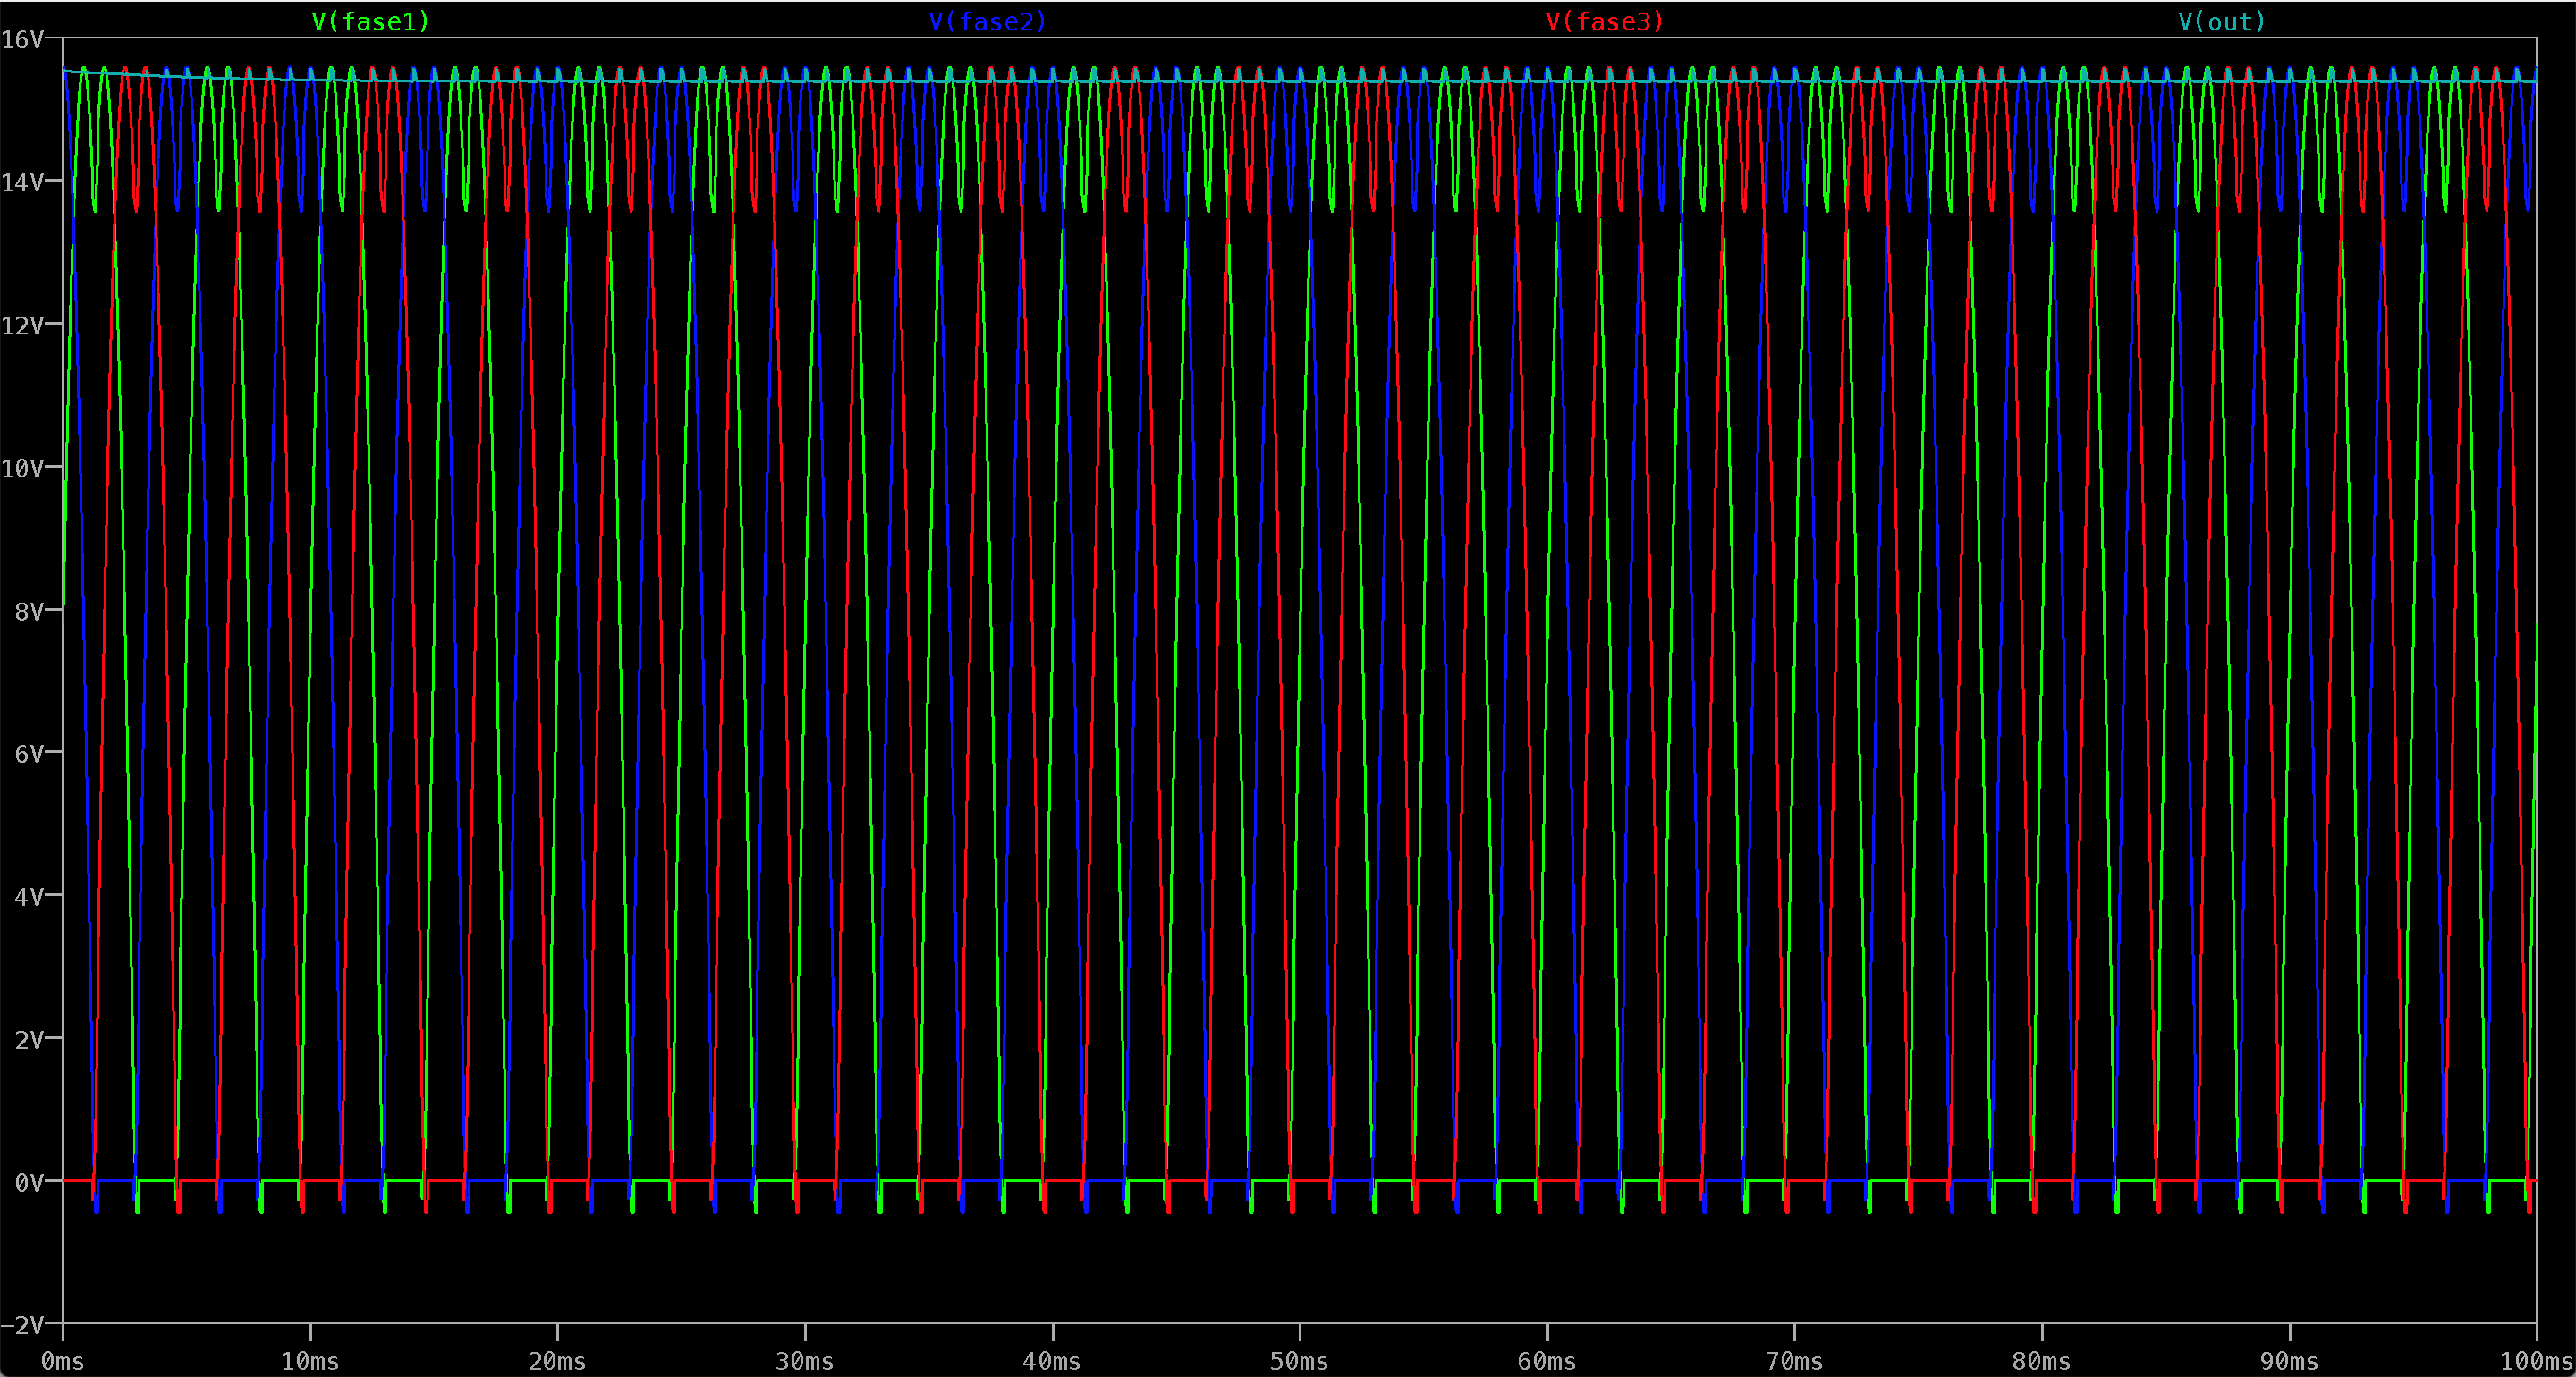
\includegraphics[width=0.6\textwidth]{real1.png}
  \caption{Resultat af simuleringen. \textcolor{cyan}{$V_{out}$: Målingen over load modstanden}, \textcolor{green}{$V_{fase1}$: Målingen af fase 1}, \textcolor{blue}{$V_{fase1}$: Målingen af fase 2}, \textcolor{red}{$V_{fase1}$: Målingen af fase 1}}
  \label{fig:real1}
\end{figure}

Som det ses i figur~\ref{fig:real1} bliver outputtet fra kredsløbet ensrettet. Der forekommer ripple på outputsignalet, men dette kan reduceres yderligere ved bedre skalering af load kondensatoren. 

Ud fra resultatet simuleringen er vi overbevist om, at ensretteren i teorien kan leve op til den ønskede funktionalitet. Derfor arbejdes der videre med realiseringen i en skaleret version. 
\clearpage
\section{Aktiv ensretter}
\label{sec:aktiv-ensretter-1}

Ud fra dette kredsløb vi har simuleret, er vi gået videre med at bygge kredsløbet på breadboard dog med en nedskalering af mosfet, da dem der er, vist i simulering ikke er til rådighed. Og da vi ikke ønsker at trække en for stor strøm igennem vores breadboard. Derfor har vi valgt en load modstand på 1kOhm. Da vil strømmen blive $\frac{V_{out}}{\mathrm{modstand}}$, så max strømmen vil ikke kunne komme over 40 mA.

\begin{figure}[h]
  \centering
  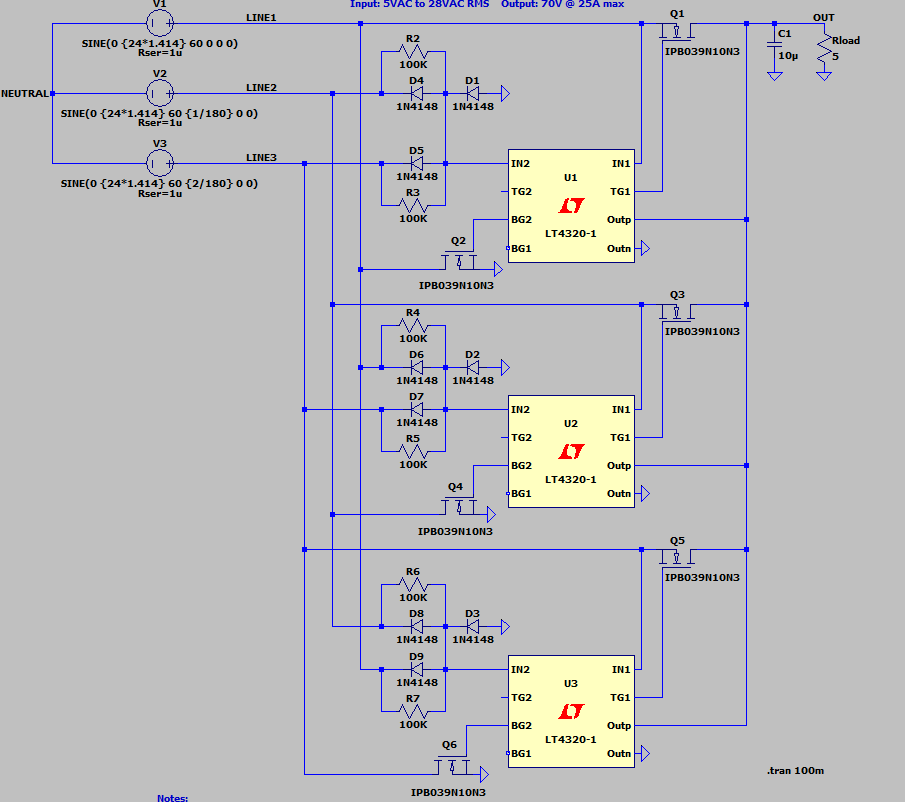
\includegraphics[width=0.6\textwidth]{schem2.png}
  \caption{Kredsløb fra simulering}
  \label{fig:schem2}
\end{figure}

Ved nedskaleringen valgte vi at bruge en mosfet ZVN2110A, den kan fint håndtere den strøm vi ønsker at trække. Dog har den en meget høj modstand i RdsON på 4 $\Omega$, som fremgår af datasheet. Det vil selvfølgelig betyde at der absorberes en højere effekt i mosfet, hvilket ikke er ønsket. Ved power mosfet som vi skal bruge ligger RdsON mellem 3-5 m$\Omega$, hvilket giver en lav effekt afsætning i komponenten.
\begin{figure}[h]
  \centering
  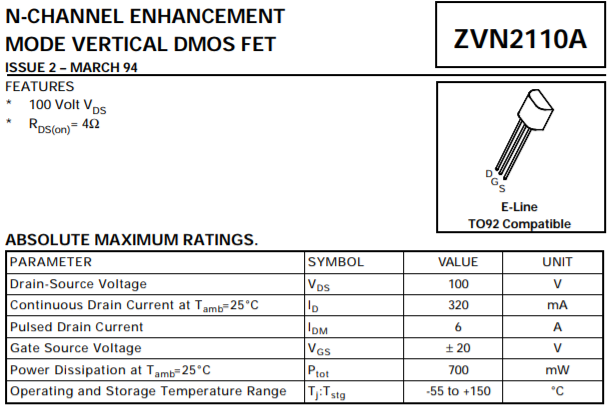
\includegraphics[width=0.3\textwidth]{pic2.png}
  \label{fig:schem2}
\end{figure}
\clearpage
\subsection{Realiseringen m/nedskalering}
\label{sec:real-mnedsk}

Nedenfor vises kredsløbet bygget på breadboard, dog har vi monteret en load kondensator på 1000$\mu$F, så vores output bliver uden rippel. Størrelsen på denne kan selvfølgelig beregnes ud fra hvor stor en strøm og ripple man ønsker. Ud fra formelen fra databladet på lt4320-1.

\begin{figure}[h]
  \centering
  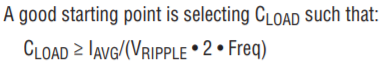
\includegraphics[width=0.3\textwidth]{formel.png}
  \label{fig:formel}
\end{figure}

\begin{figure}[h]
  \centering
  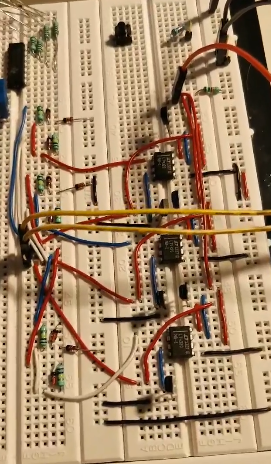
\includegraphics[width=0.4\textwidth]{bread1.png}
  \caption{Breadboard med aktiv ensretter}
  \label{fig:bread1}
\end{figure}

\subsection{Målinger}
\label{sec:malinger}

Første måling vises der de tre faser og spændingen over load modstanden. Alle målinger blev målt med reference til ground på load modstanden.
\begin{itemize}
\item Channel 1: er output på load modstanden
\item Channel 2,3,4: er de tre faser.
\end{itemize}

På billedet kan der aflæses max peak værdi, ude til højere under ”Measurements”. Her ses at vores output næsten har samme spænding som på faserne, hvilket er godt da, dette betyder meget lidt effekttab i kredsløbet.

\begin{figure}[h]
  \centering
  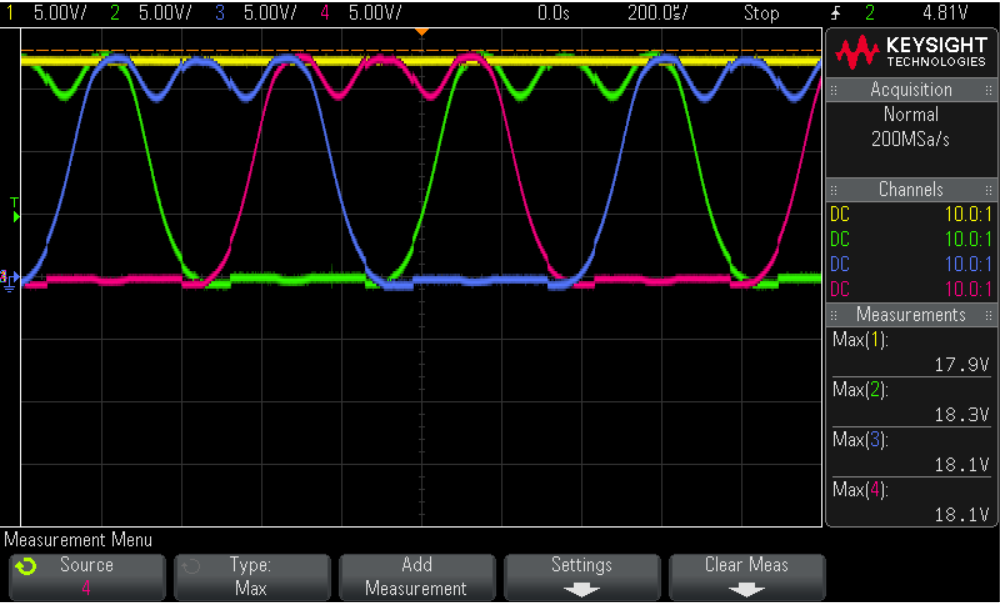
\includegraphics[width=0.6\textwidth]{graf1.png}
  \label{fig:graf1}
\end{figure}

For at kunne bevise at dette kredsløb er væsentlig bedre end en diode bro, valgte vi at måle på spændingen på gaten på mosfet. I forhold til fasen, den skulle gerne være under 0,7 volt, da dette er forward voltage på en diode. Ellers er den ikke bedre end en diode bro.

\begin{figure}[h]
  \centering
  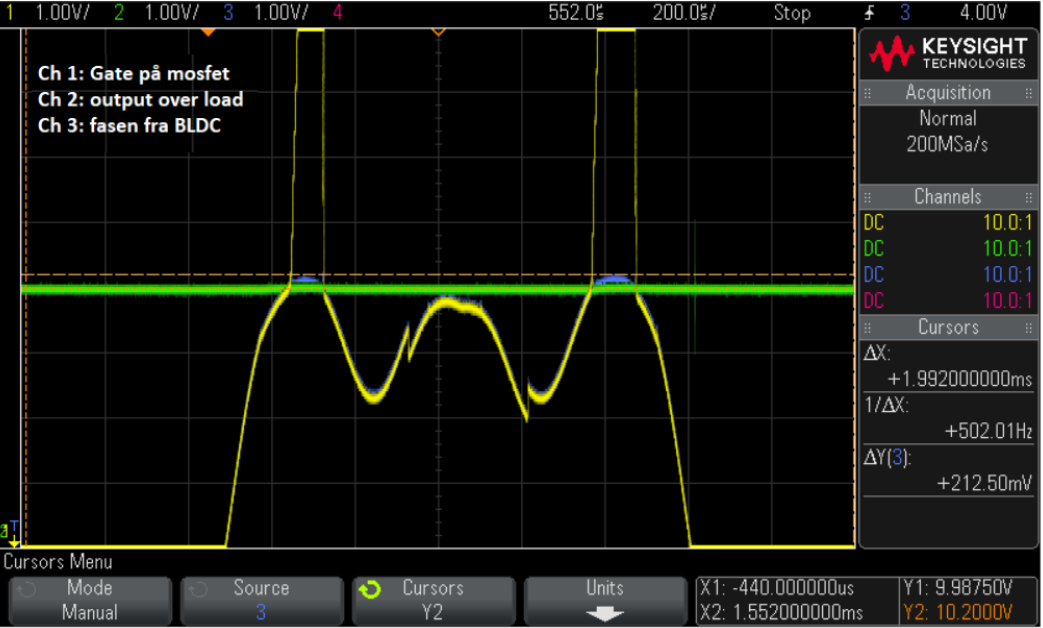
\includegraphics[width=0.6\textwidth]{graf2.png}
  \label{fig:graf2}
\end{figure}

Resultatet er spændingen kun er 212.50 mV. Dette beviser at vores kredsløb er væsentlig bedre end en diode bro. Dog kunne denne spænding bliver mindre endnu, grunden til dette er vores mosfet som har en modstand på 4 ohm ’RdsON’. Hvilket giver et lidt større spændingsfald. Denne modstand bliver som nævnt tidligere også reduceret væsentlig ved udskiftning af komponenten. Dette resultere i en endnu mindre effekt tab i vores mosfet.
\clearpage

\section{Motorstyring (Simon)}
\label{sec:motorstyring}

I denne timebox fremlægges design af teststand for præcision af koefficienter i PID-regulering. For at simplificere PID-reguleringen forsøges forst med regulering af spjæld i forhold til motorens omdrejninger. Der vil tages udgangspunkt i måling af et steprespons på motorens omdrejninger. Til målinger af omdrejninger foreslås at bruge Pocketbeagle som vil kunne foretage måling af omdrejninger via Hall-sensor og lagre data i en fil som kan eksporteres til analyse i Matlab.

Udfra stepresponset noteres

\begin{itemize}
\item Rise time, $t_r$
\item Settling time, $t_s$
\item Overshoot, $M_p$
\item Peak time, $t_p$
\end{itemize}

Udfra disse mål kan der gives et bud på en overføringsfunktion. I matlab kan der via simulink og en overføringsfunktion findes PID-koefficienter og laves tuning. I slutningen af arbejdet undersøges om følgende kravene overholdes:
\begin{itemize}
\item Overshoot skal ikke være mere en 197 rpm.
\item Justeringstiden må max være 8,8 sekunder.
\item Ifm. et step respons skal 90 \% af målet være opnået i mindre end 3 sekunder.
\end{itemize}

I næste timebox skal de fundne PID-koeffiecienter implementeres og det skal undersøges om kravene overholdes. Evt. kan der afprøves med stepresponser af tilgrænsende koeffecientværdier for at undersøge om PID-reguleringen kan optimeres yderligere.


\section{Deployment (Alle)}
\label{sec:deployment}

Hermed godkender kunderne, Morten Oppbrud Jakobsen og Jan Møller Nielsen, ovenstående i timebox 7.

Mandag den 1/4-2019

\begin{minipage}{.5\textwidth}
  \begin{center}
    \vspace{1.4cm}
    \rule{0.8\textwidth}{0.1pt}\\
    \small{Morten Opprud Jakobsen\\%\vspace{0.1cm}\textit{Projektansvarlig læge}
    }
  \end{center}
\end{minipage}%
\begin{minipage}{0.5\textwidth}
  \begin{center}
    \vspace{1.4cm}
    \rule{0.8\textwidth}{0.1pt}\\
    \small{Jan Møller Nielsen\\%\vspace{0.1cm}\textit{Forskningsansvarlig overlæge}
    }
  \end{center}
\end{minipage}

% \printbibliography
\end{document}